\documentclass{article}
\usepackage{graphicx}
\usepackage{listings}
\graphicspath{ {images/} }

 \pagenumbering{arabic}
 \usepackage{array}
 





\begin{document}


\includegraphics[width=10cm, height=5cm]{logo} \break \break

\centering {\textbf{Computer Science and Engineering} }\\

 \centering{A.A. 2016/2017} \\
\centering{Software Engineering 2 Project:} \\

\centering{\textbf{ Power\&Joy} }\break



\centering{\textbf{\large{Requirements Analysis and Specification Document}} }\break \break

\centering{November 11, 2016 }\break





\begin{flushright}


Prof. Luca Mottola\break 
Joshua Nicolay Ortiz Osorio \ Mat: 806568 \\
Michelangelo Medori \ Matr: 878025

\end{flushright}

\newpage

\centering {\textbf{Index}} \\    %INDEX
\begin{enumerate}

\item Introduction




\begin {enumerate}
\item [1.1] Purpose
\item [1.2] Descriprtion of the given problem
\item [1.3] Stakeholders
\item [1.4] Glossary
\item [1.5] Reference documents
\item [1.6] Overview
\end{enumerate}

\item Ovrall Description
\begin {enumerate}
\item [2.1] Product Perspective
\item [2.2] Actors Identifying
\item [2.3] Goals (Product Functions)
\item [2.4] Domain Properties
\item [2.5] Text Assumprtions
\item [2.6] Constrains 
\end {enumerate} 


\item Specific Requirements
\begin {enumerate}
\item [3.1]  Functional Requirements
\item [3.2] Non Functional Requirements
\item [3.3] Mockups

\end {enumerate} 


\item UML Models
\begin {enumerate}
\item [4.1] Use case Diagram
\item [4.2] Activity Diagrams
\item [4.3] Class Diagrams
\item [4.4] State Diagrams
\item [4.5] Sequence Diagrams

\end {enumerate} 


\item Alloy
\begin {enumerate}
\item [5.1] Model  
\item [5.2] World Generated

\end {enumerate} 


\item Other Features
\begin {enumerate}
\item [6.1] Future Development
\item [6.2] Used Tools
\item [6.3] Hours of Work

\end {enumerate} 

\end{enumerate}

\newpage

\begin{flushleft}\section{Introduction}    %INTRODUCTION
\subsection{Purpose}%PURPOSE
This is the first of a series of documents aimed to project a digital management system for a car sharing service. Identifying stakeholders, modeling scenarios and formalizing requirements and constrains of the system are the main topics of this document.

\subsection{Descriprtion of the given problem}%DESCRIPTION OF THE GIVEN PROBLEM
We are going to design a digital management system for a car sharing service that only employs electric cars (i.e. cars powered by rechargeable batteries), which are environment-friendly and noise-free.?Precisely, we want to offer the possibility to users to choose a car among an amount of cars dislocated into Milan's urban area, to travel across the city.?Electric cars gather their fuel when they are plugged into proper power grids; these grids are placed all around the city: they can be found into specific charging stations, beyond near a decent number of parking lots around Milan.?Cars can be parked everywhere inside Milan urban area (i.e. any kind of appropriate car park, accordingly to Italian laws, including pay and display parking lots). ?Operators are available to make sure that cars are never left with less than 20\% battery charge by charging them into near charging stations or in place.?The final aim of the system is to provide a service within anyone's reach, that stands for a solid alternative to public transport.
\subsection{Stakeholders} %STAKEHOLDERS
The only stakeholders that we have is Power\&Joy society that require the management system of car sharing.
\subsection{Glossary}%GLOSSARY
\begin{itemize} 
\item \textbf{System:} is the system we will create which is going to manage the car sharing service. The system has a dedicated database where it can store and access all needed information.
\item \textbf{User :} every person registered into the system that wants to use a car.
\item \textbf{Not Register User (NRU) :} all people not registered in the system.
\item \textbf{Operators:}  employees working on charging stations whose job is recharge every car that has less 20% battery level and to provide assistance to the users.
\item \textbf{Passenger :} a person who is traveling in a car (included the driver). 
\item \textbf{Registration (for Users): } consists in the act of inserting all the needed information into the system as
\begin {itemize}
\item First name and Last name
\item E-mail
\item Password
\item Phone number
\item Birth date 
\item ID card code 
\item Drive license code


\item Credit card number 
\item Fiscal code
\end{itemize}



\item \textbf{ Safe Area: } Milan?s urban centre.
\item  \textbf{Power grid station:} a stopping place for electric cars equipped with electric socket and where operators work.
\item \textbf{Available car:} is a car that is not currently used by other users and has the battery charge level over 20%.
\item \textbf{Parking lot:} every available car park inside the Safe Area that respects the Italian traffic laws.
\item  \textbf{Special Parking lot:} every parking lot equipped with electric socket.
\item  \textbf{Safe Zone: }is a circular zone with 3 km of diameter which centre is a power grid station.
\item  \textbf{Reservation:} is the ability to reserve a car for at maximum 1 hour, then the reservation expires.
\item  \textbf{Contactless  card: }card acquired by users at the moment of the registration used to unlock the reserved cars.
\item  \textbf{Special contactless card:} Magnetic card acquired by operators at the moment of the registration that can be used to unlock any car.
\item  \textbf{Unlock Car:}  to undo the lock of car?s doors  by  placing the contactless cards or special contactless cards near specific sensors placed over the car doors.
\item  \textbf{Password: }is the key to log in to the system.
\item  \textbf{Status (of a car):} any of the possible conditions of the cars (low  charge/assistance needed/accident/no issues). 
\item  \textbf{Reserved Operator area:} special section of the system where operators can register and log in, and from which they can access information about the position and the status of all the cars.
\item  \textbf{Ride: }it starts one minute after the user unlocks the car and ends when the user shuts down the car and pushes on the display ?end the ride? button.
\item  \textbf{Pit Stop:} it happen when the user stops the car for a short period of time (maximum 60 minutes) and keep  the car reserved in order to continue the ride.
\item  \textbf{End the ride:} user stops the car, leaving it in a safe parking lot so that the car is made available for other reservations by other users.
\item  \textbf{Scalability: }is the capability of a system, network, or process to handle a growing amount of work, or its potential to be enlarged in order to accommodate that growth.
\item  \textbf{Quality of Service:} �is the overall performance of a computer network, particularly the performance seen by the users of the network. His attributes are: Performance, Reliability, Scalability, Capacity, Accuracy, Availability, Robustness, Integrity and Confidentiality.
\item  \textbf{On-board computer:} a computer equipped with a touch screen and a GPS navigation device, placed in every car. It can also perform calls (in particular, it can perform accident calls, as defined below).
\item  \textbf{CID module: }a document that must be filled in case of accident by the people involved with the accident details (according to Italian traffic laws)
\item  \textbf{Assistance call: }call made by an user from his phone to ask for assistance about how to use the cars. These calls are picked up by the call center
\item  \textbf{Call center:}  place where assistance calls are picked up by operators. The only  job of the operators who work on the call center is to pick up assistance call (they do not provide physical assistance to users). Call center is NOT equipped with power grids.
\item  \textbf{Accident calls:} calls automatically started by the on-board computer when a user taps on the ''REPORT ACCIDENT'' button on the on-board computer. 
\item  \textbf{Card ID:} a number associated to each operator (written on their contactless card) that identifies them

\end{itemize}

\subsection{Reference documents} %REFERENCE DOCUMENTS
These are the documents we used as guideline:
\begin{itemize}
\item Specification Document: Assignment AA 2016-2017 (RASD)
\item IEEE Std 830-1998 IEEE Recommended Practice for Software Requirements Specifications.
\item Examples Documents: RASD sample from Oct. 20 lecture.
\end{itemize}
\subsection{Overview} %OVERVIEW
After a short description of the system?s properties, we define goals (e.g. the functions the system has to be able to perform)  and constrains, and make assumptions that we suppose hold in the analyzed world. Then we analyze and formalize the goals with the help of UML diagrams (use case, sequence diagrams, class diagram) and the formal language Alloy. 

\section{Overall Description} %OVERALL DESCRIPTION
\subsection{Product Perspective} %PRODUCT PERSPECTIVE
We want this service to be accessible via mobile or web app. Every user (i.e. person who wants to reserve and ride a car)  must register to the system via the mobile or web app providing general information (full name, age, e-mail etc.) and specific ID's (fiscal code, drive license code). Once registered and logged in,  the system allows user to view on a map the current geographical position of every available car, thanks to GPS sensors on each car. Cars already in use by other users do not display, but the system can access the information about the positions and the batteries of every single car, weather they are being used or not, any time it needs to (in case of assistance requests et al.).\\??Users can choose a car at the time, and make a reservation for it. They shall reach the car within 60 minutes from the moment the reservation is made,  to be able to use the car.?When near, users can unlock the car by simply placing  their contactless card  (provided at the moment of the registration) near the sensor placed on the car door.?The system unlocks the car soon after and the user is able to get in. In order to start the ride, the user simply needs to turn the key  placed inside the car. 
Every car is equipped with an on-board computer, that can be used to communicate the existence of damages over the car as well as GPS navigator device.?Before starting the ride, the system encourages the user to make sure the car is not damaged or compromised, and to communicate it, in case issues are found, via the mobile app or the on-board computer.
Once the car is started, the user starts to be charged per minute of ride.\\?Once they end the ride, users can park cars in every available car park inside the urban area (which includes any kind of parking lot, accordingly to Italian laws, pay and display car parks included, private parking lots excluded).  ?Some special parking lots are equipped with power grids to recharge the car, and discounts are available in case users take care to plug the car in.?Discounts are also available in case the user leaves the car with more than 50\% battery charge or if he takes on the ride 2 more passengers , while the user is going to pay 30\% more of the price of his ride in case he leaves the car with 20\% battery charge or more than 3 km away from the nearest charging station.\\?Payments are always carried out through the credit card that the user has to insert at the moment of the registration and a receipt is available to view with the mobile app or via e-mail.
A group of operators is available to give assistance to users and to make sure cars are never left under 20\% battery charge. Operators work at charging stations and can access all the information about cars positions and batteries. \\

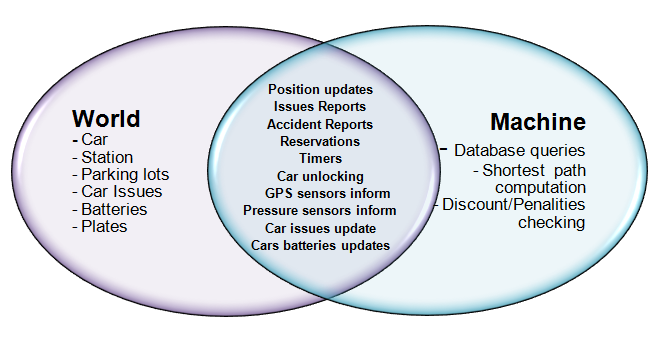
\includegraphics[width=10cm, height=5cm]{worldmachine} 

\subsection{Actors Identifying} %ACTORS IDENTIFYING
There are two main kind of people the System needs to interact with:
\begin {itemize}
\item Users
\item Oprators

\end {itemize}
Both of them need to be registered into the system.?Operators work at the charging stations and need to pick up and recharge every car below 20% battery charge and provide assistance to users, if needed.?The goals concerning  the interaction between these two groups of people and the system are described below.

\subsection{Goals (Product Functions)} %GOALS
\flushleft{ \textbf{Users:}}\\
\begin{enumerate}
\item The system shall allow users to register via the web or mobile app by inserting all the required information
\item The system shall allow users to log in
\item The system shall allow users to see the positions of all the available cars on a map
\item The system shall allow users to make a reservation for an available car
\item The system shall allow users who reserved a car to cancel the reservation
\item  The system shall allow users to unlock the car they reserved
\item The system shall allow users to start the ride
\item The System shall allow users to make a pit stop of maximum 60 minutes
\item The system shall allow users to end the ride only if the car is parked inside the safe area
\item The system shall allow users to communicate if the car they reserved is damaged or issues are found (e.g. dirt, damages, etc.)
\item The system shall compute the price of every ride taking into account discounts and penalties and send it to the system which takes care of the payment
\item The system shall allow users to report an accident via the on-board computer

\end{enumerate}


\flushleft{ \textbf{Operators:}}\\
\begin{enumerate}
\item The system shall allow operators to log into a dedicated area .
\item The system shall allow operators to view the updated status and position of every car
\item The system shall allow operators to be able to select a car from the list in order to take care of it.
\item The system allow an operator who took care of a car to communicate that the issues are resolved to all the other operators

\end{enumerate}

\subsection{Domain Properties} %DOMAIN PROPERTIES
\begin{itemize}
\item The contact-less card is received by users not later than 3 days after the registration is performed.
\item Parking a car where is not allowed by the traffic laws is subject to penalties for the user that parked it, according to Italian laws.
\item Damages found on the cars are paid by the last user before the one who signals the found damages
\item In case a user needs assistance he can call an operator with the number displayed on the window of every car
\item All cars are equipped with a GPS navigation device.
\end{itemize}

\subsection{Text Assumprtions} %TEXT ASSUMPTIONS
\begin{itemize}
\item There are no identical fiscal codes or license numbers related to different users or operators
\item The credit card inserted at the moment of the registration by the user is a valid (existing and working) one
\item Users only register into the system once
\item The user who unlocks the car is the owner of the contact-less card he uses and is the same who is actually going to drive that car
\item Cars are equipped with GPS sensors in order to be localized by the system
\item Cars are equipped with pressure sensors on every seat, in order to let the system know exactly how many passengers are onto the car anytime
\item Users start the ride after at maximum 1 minute after they unlock the cars
\item Users will not leave the car in a zone where is not possible to detect the GPS sensor, even if it is inside the safe area
\item Users do not leave cars into private parking lots
\item User will not perform any kind of maintenance or reparation operations to the car 
\item User will not  leave the car in any kind of condition which could cause damage or any  issue on the surrounding area.
\item Users will not try to leave cars outside the safe area.
\item Users will not try to reserve more than a car at once
\item The credit card  used by the users always has enough money to pay for the rides
\item Users will always leave the car with the windows closed, handbrake activated, lights  and radio off and all the documents stored in their right place  at the end of every ride
\item Users will always instantly receive, after they end a ride, the information about the ride itself via e-mail and the mobile app. These information include time and money  spent, distance traveled , etc
\item All the payments are correctly performed at the end of every ride
\item In case of issues on a car, users always notice them and notify it to the system before starting the ride
\item If an operator taps the button ''OPERATE'' associated to an issued car, he actually performs all the needed actions in order to fix that car within 4 hours , and always remembers to tap the button ''ISSUE SOLVED'' once they finished
\item Operators are registered into the system and all their data is stored onto the database. The information inserted by operators at the moment of the registration is always consistent
\item Operators have a special section of the system where they can log and access all the information they need to perform their job. They can log using a password chosen during the registration
\item Operators  working on the call center are always available to pick up calls from users who need assistance 
\item The assistance number users can call is written on the window of every car, and is visible both from inside and from outside the car
\item The number used for accident calls is different from the one used for assistance calls, and is not available for user to call unless they tap on the ''REPORT ACCIDENT'' on the onboard computer
\item User only tap the ''REPORT ACCIDENT'' on the on-board computer if they were actually involved in an accident
\item Once a user makes an accident call, the call is redirected to the nearest charging station, and always instantly picked up by an operator.
\item Once a user makes an accident call, an operator always  reaches the place of the accident in less than 15 minutes
\item If the presence of a passenger is detected by the sensor at the beginning of the ride as well as at the end, the system supposes that the passenger has been on the car for the whole ride.
\item User only pay for damages found on the cars if they actually performed those damages
\item Accident calls are picked up by operators who do not work on the call center (only charging stations)
\item Operators have a special contact-less card they can use to unlock the cars, acquired at the moment of the registration into the system
\item Operators can drive any car unlocking them via the special contact-less card, and without  paying for the ride
\item In case of accident the user always takes care of stopping the car in some place where it doesn?t create problems to the traffic flow, never panics, fills the CID modules (according to Italian laws)  and remains in the place where the accident happened until the arrive of the operator
\item In case users leave any kind of items into the cars after ending the ride, they can inform operators about that via a phone call, and operators will pick their stuff; users will collect it in one of the charging station

\end{itemize}
\subsection{Constrains} %CONSTRAINS
\begin{itemize}
\item The implementation language must be Java
\item The credit card payment system must be able to be dynamically invoked by other systems relying on it
\end{itemize}
\flushleft{ \textbf{Network connections:}}\\
Power\&Joy webApp needs internet connection for working. In particular if a user needs to make a reservation or cancel it , he has to switch on 3G  or LAN wireless connection. \\

\flushleft{ \textbf{Concurrent operations}}\\
The system has to guarantee multiple processes from different connected users.\\
\flushleft{ \textbf{Hardware limitations}}\\
All the mobile phone must have GPS to localize and reach the cars. They required a space for App package too.\\

\flushleft{ \textbf{Interfaces to other applications }}\\
The system will interface with a new  MySQL database. All the information about users and operators are saved here and the system through queries can use them.\\


\section{Specific Requirements} %SPECIFIC REQUIREMENTS
\subsection{Functional Requirements} %FUNCTIONAL REQUIREMENTS
\begin{enumerate}
\item \textbf{The system shall allow users to register via the web or mobile app by inserting all the required information}
\begin{enumerate}
\item The system requires to insert all personal information that consist on : 
\begin{itemize}
\item First name and Last name
\item E-mail
\item Password
\item  Phone number
\item Birth date 
\item ID card code
\item Drive license code 
\item Credit card number 
\item Fiscal Code
\end{itemize}


\item The system shall check that all information inserted are valid (e.g. all text boxes must be not empty, the name cannot contain numbers etc).
\item The system includes the information of the new user onto the database
\item The system sends a confirmation e-mail to the new user.
\end{enumerate}

\item \textbf{The system shall allow users to log in}
\begin{enumerate}
\item In order to log in, the system shall require users to insert their credentials (consisting of an e-mail/username and a password) into an input form  accessible from the web or mobile app.
\item The system shall verify that the credentials are valid , and only in that case give access to the area where cars positions are displayed.
\item n case the credentials are not valid, the system shall negate the access  

\end{enumerate}

\item \textbf{The system shall allow users to see the positions of all the available cars on a map}
\begin{enumerate}
\item The car are equipped with a GPS sensors that allow the system to localize them anytime.
\item The system puts all the cars positions on a map that can be visualized by users via web or mobile application.
\item The user shall be able to insert a specific address or geographical position, in order for the system to show the available cars around the wanted location.
\item The system shall allow users to view all the positions of the cars which are strictly placed around users current position by simply tapping a button on the app. This is only possible if GPS sensor are working on the device the user is utilizing to view the map.
\end{enumerate}

\item \textbf{The system shall allow users to make a reservation for an available car}
\begin{enumerate}
\item When the user finds a suitable car he can reserve it by clicking on the ?RESERVE? button on the application.
\item After doing the reservation the system starts a timer of 60 minutes.  If the user is not able to unlock  the reserved car before the time expires, the system cancels the reservation making the car available again for other users.?
\end{enumerate}

\item \textbf{The system shall allow users who reserved a car to cancel the reservation}
\begin{enumerate}
\item Once a user reserved a car, the system shall allow him to cancel the reservation for it before the timer of 60 minutes expires by clicking on a button ''CANCEL RESERVATION'' on the mobile or web app.
\item If the user cancels a reservation, the system shall  make the car available again for other users.

\end{enumerate}

\item \textbf{The system shall allow users to unlock the car.}
\begin{enumerate}
\item Any  reserved car can only be unlocked using the contactless card owned by the user that reserved that specific car, and before the timer of 60 minutes expires. 
\item When the user places the contactless card near the sensor of the car, the system  shall acquire information about the card, verify that it corresponds to the user that actually reserved that car and, in that case, the system shall unlock the car in order for the user to get in
\item In case the contactless card is not recognized as valid by the system, the system denies access to the car, until a valid card is recognized by the time the timer expires.

\end{enumerate}

\item \textbf{The system shall allow users to communicate if the car they reserved is damaged or issues are found (e.g. dirt, damages, etc.).}
\begin{enumerate}
\item Before starting the engine the system shall remind the user through the on-board computer to check  for damages on the car and to communicate it in case issues are found via the mobile  app or the same on-board computer
\item In case of issues, the system shall cancel the reservation , make the car unavailable for users, marking it as ''ASSISTANCE NEDEED'' in order to inform all operators.

\end{enumerate}

\item \textbf{The system shall allow users to start the ride.}
\begin{enumerate}
\item In order to start the engine the user shall turn the key.
\item The system shall start to charge the user by minute of ride as soon as he ignites the car engine.
\item The system shall display on the onboard computer the updated amount of money spent for the ride.

\end{enumerate}

\item \textbf{The System shall allow users to make a pit stop of maximum 60 minute.}
\begin{enumerate}
\item The system shall allow users to make a pit stop of maximum 60 minutes communicating it tapping a button ''START PIT STOP'' on the onboard computer. When they do it, the system starts a timer of 60 minutes.
\item When the user wants to end the pit stop he needs to tap again a button ''END PIT STOP'' on the onboard computer, or simply restarting the car.
\item During the pit stop the system shall still go on charging users for 50\% of the price during all the time the pit stop lasts or since the timer expires.
\item During the pit stop the system shall always make the car stay reserved for the current user, and unavailable to other users.
\item When the Timer expires the system cancels the reservation for that car, making it available for other users to use.
\end{enumerate}

\item \textbf{The system shall allow users to end the ride only if the car is parked inside the safe area.}
\begin{enumerate}
\item When the user wants to end the ride, he has to communicate it to the system by tapping a button ''END THE RIDE'' on the onboard computer.
\item The system shall check if the car is parked inside the safe area using the GPS sensor information, and only in that case  allow user to end the ride.
\item If the car is not parked into a safe area, the system shall go on charging users until they move the car inside the safe area  and tap the button ''END THE RIDE'' on the onboard computer.
\item The button ''END THE RIDE'' shall  only be available to press if the car engine is shut down.
\end{enumerate}

\item {\textbf{The system shall compute the price of every ride taking into account discounts and penalties and send it to the system which take care of the payment.}}
\begin{enumerate}
\item When a ride ends (if the users taps the ''END THE RIDE '' button while the car is parked inside the safe area ,or if  the pit stop timer of 60 minutes expires) the system shall compute the total cost of the ride using the price currently displayed on the on-board computer and taking into account the following rules:
\begin{itemize} 
\item If the system detects the user took at least two other passengers onto the car, the system applies a discount of 10\% on the last ride. In order to detect the presence of a passenger, the system shall check that the pressure sensors of the car seats are active both at the beginning and at the end of the ride.
\item At the end of the ride, the system shall check the battery charge: if a car is left with no more than 50\% of the battery empty, the system applies a discount of 20\% on the ride. 
\item At the end of the ride, the system shall check if a car is left plugged into one of the power grids available through the charge sensor: in that case the system applies a discount of 30\% on the last ride.
\item At the end of the ride the system shall check if a car is left at more than 3 KM from the nearest power grid station or with more than 80\% of the battery empty, the system charges 30\% more on the  ride (in order to do that, the system shall compute the shortest path from the final position of the ride to all the charging stations, find the minimum one and compare it with 3km).
\end{itemize}
\end{enumerate}

\item {\textbf{The system shall allow operators to log into a dedicated area .}}
\begin{enumerate}
\item In order to log in, the system shall require operators to insert their credentials (consisting of an e-mail/username and a password) into an input  form  accessible from the web or mobile app.
\item The system shall verify that the credentials are valid , and in that case give access to the dedicated area.
\item In case the credentials are not valid, the system shall negate the access

\end{enumerate}

\item {\textbf{The system shall allow operators to view the updated status and position of every car }}
\begin{enumerate}
\item Once they are logged in , the system shall allow operators to view (via web or the mobile app) the positions of all the cars on a list, associating to each car a status:      ''NO ISSUES''  is for charged (or currently on charge) and working cars, ''LOW CHARGE''  is for cars under 20\% battery charge, ''ASSISTANCE NEEDED'' is for cars that need some kind of maintenance or reparations, ''ACCIDENT'' in case a user is involved in a car accident while riding the car.
\item The system shall always keep all the positions and the status of the cars updated

\end{enumerate}

\item {\textbf{The system shall allow operators to be able to select a car from the list in order to take care of it.}}
\begin{enumerate}
\item Operators shall be able to communicate to the system they are taking care of a car by selecting a row on the list and tapping a button ''OPERATE''.
\item Once an operator pressed the '' OPERATE''  button on a row of the list  corresponding to a car, the system shall deny other operators to take care of the very same car, substituting the ''OPERATE'' button with a writing ? in progress..? (this is only valid for all the operators except the one that is taking care of the car, to whom another kind of button is displayed by the system, as described below)

\end{enumerate}

\item{ \textbf{The system allow an operator who took care of a car to communicate that the issues are resolved to all the other operators}}
\begin{enumerate}
\item Once issues are resolved for a specific car , the specific operator who took care of it, shall be able to communicate it to the system by tapping a ''ISSUES SOLVED?''button (only available to the operator who pressed the ''OPERATE'' button earlier). The system shall then mark the car as ''NO ISSUES'' again for all the operators.

\end{enumerate}

\item {\textbf{The system shall allow users to report an accident via the on-board computer}}
\begin{enumerate}
\item Once the ride is started, the system shall display on the on-board computer a button ''REPORT ACCIDENT''
\item In case the ''REPORT ACCIDENT'' button is pressed by a user, the system shall  stop charging the user, forcing him to end the ride and inform operators  marking the car with the ''ACCIDENT'' writing .

\end{enumerate}


\end{enumerate}




\subsection{Non Functional Requirements} %NON FUNCTIONAL REQUIREMENTS
\begin{itemize}
\item The system must be available 24 hours a day
\item The system must respect Quality of Service (QoS)  attributes .
\item The system shall start all the required timers within 1 second after the user?s input.
\item The system shall unlock the car within 5 seconds after the contactless card is placed near the car sensor
\item The system shall start charging the users within 2 seconds after they start the car engine at the beginning of a ride
\item The system shall stop charging users within 2 seconds after they tap on the ''END THE RIDE '' button on the on-board computer, having the engine shut down,  the car parked inside the safe area, and the car GPS signal available.
\item The system shall change the status of every car within 2 seconds from one of the following events:
\begin{enumerate}
\item A car switches from 20\%  to 19\%  battery charge
\item  An operator taps the ''OPERATE'' button associated to an issued car to take care of it 
\item  An operator taps the ''ISSUES SOLVED'' button associated to a car they took care of
\item A user taps on the button ''ISSUES FOUND'' on the on-board computer of a car
\item A user taps on the ''REPORT ACCIDENT'' on the on-board computer
\end{enumerate}
\end{itemize}


\subsection{Mockups} %MOCKUPS
\subsubsection {\textbf{User's log in / Operator's log in} }
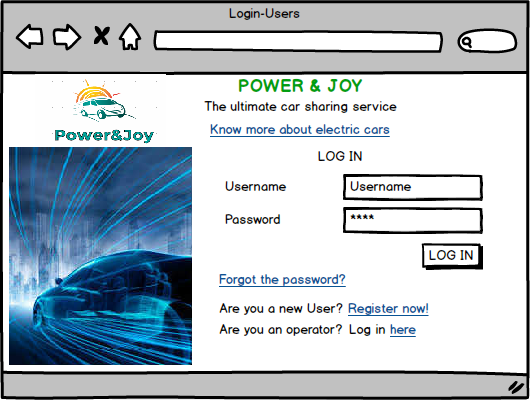
\includegraphics[width=8cm, height=6cm]{m1}
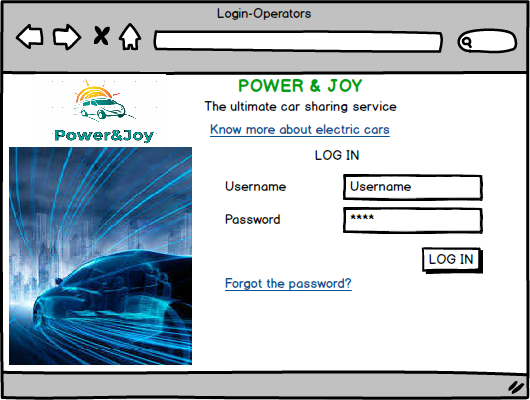
\includegraphics[width=8cm, height=6cm]{m2}  

\subsubsection {\textbf{Users Registration/ Users Home Page / Reservation Countdown} }
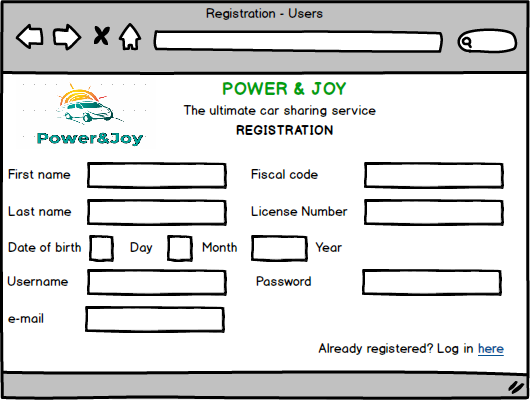
\includegraphics[width=8cm, height=6cm]{m3}
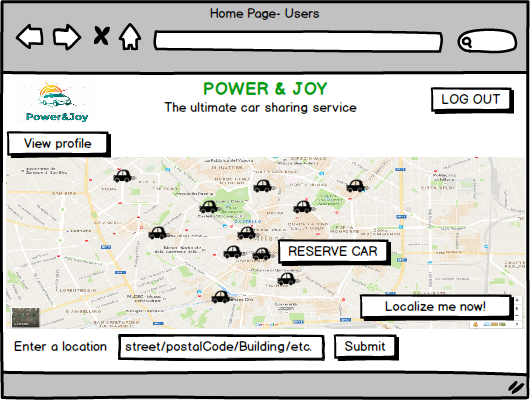
\includegraphics[width=8cm, height=6cm]{m4}  
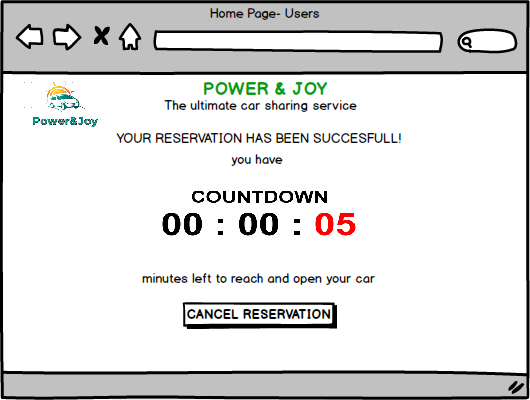
\includegraphics[width=8cm, height=6cm]{m5}  

\subsubsection {\textbf{Operator's Home Page} }
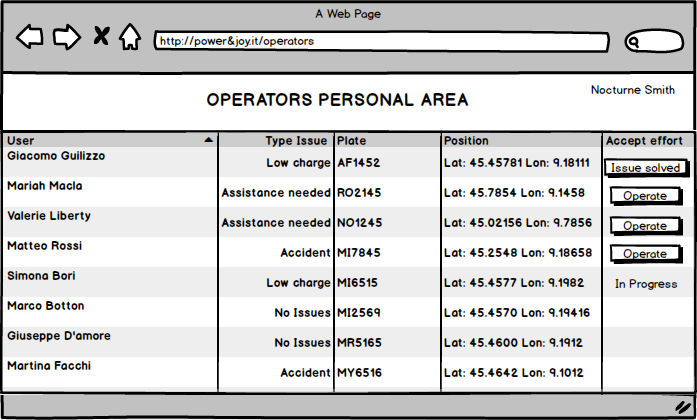
\includegraphics[width=8cm, height=6cm]{m6}

\subsubsection {\textbf{Mobile: User log in / User Home Page} }
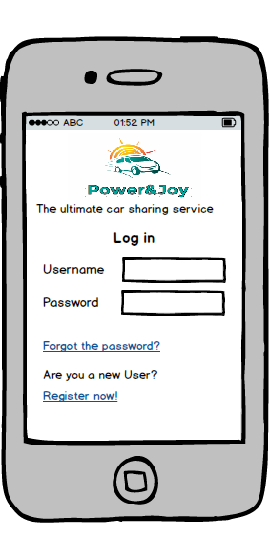
\includegraphics[scale=0.5]{mm1}
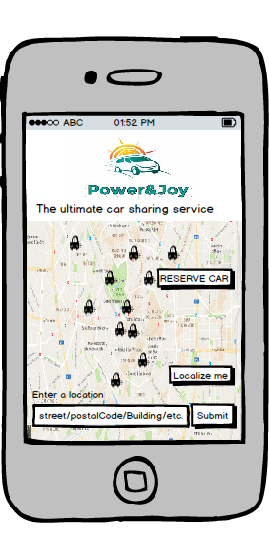
\includegraphics[scale=0.5]{mm2} 

\subsubsection {\textbf{Mobile: Reservation Countdown / Operators Home Page} }
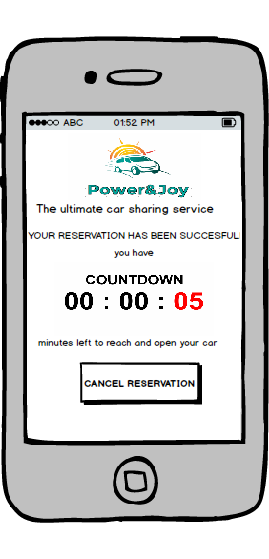
\includegraphics[scale=0.5]{mm3}
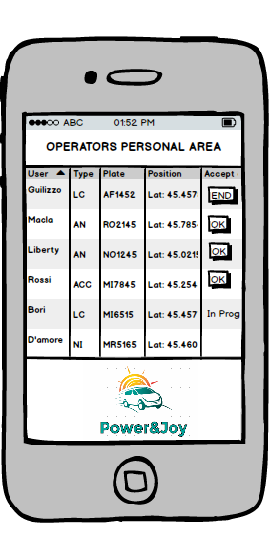
\includegraphics[scale=0.5]{mm4} 

\subsubsection {\textbf{On-Board Computer:  Signal Issues / Map} }
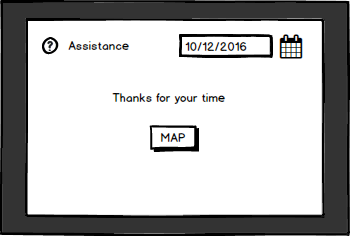
\includegraphics[width=8cm, height=6cm]{mob1}
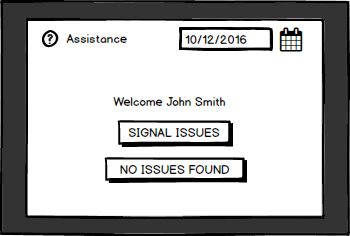
\includegraphics[width=8cm, height=6cm]{mob2} 

\subsubsection {\textbf{ On-Board Computer: Start Pit Stop / End Pit Stop}}
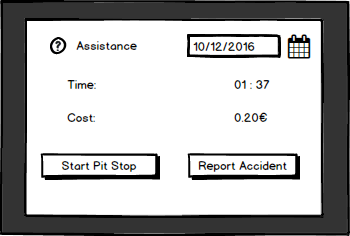
\includegraphics[width=8cm, height=6cm]{mob3}
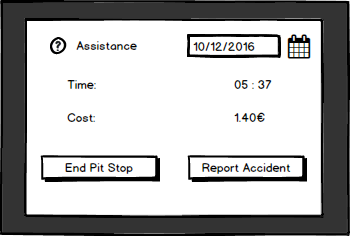
\includegraphics[width=8cm, height=6cm]{mob4} 

\subsubsection {\textbf{ On-Board Computer: End the ride}}
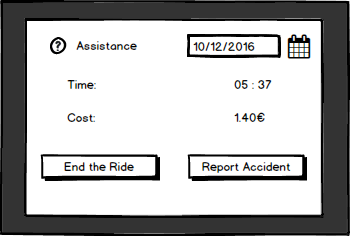
\includegraphics[width=8cm, height=6cm]{mob5}
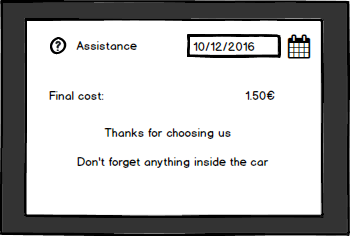
\includegraphics[width=8cm, height=6cm]{mob6} 

\subsubsection {\textbf{ On-Board Computer: Report accident}}
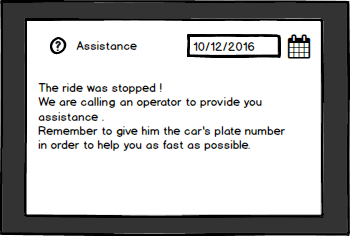
\includegraphics[width=8cm, height=6cm]{mob7}

\section{UML Models} %UML MODELS
\subsection{Use case Diagram} %USE CASE
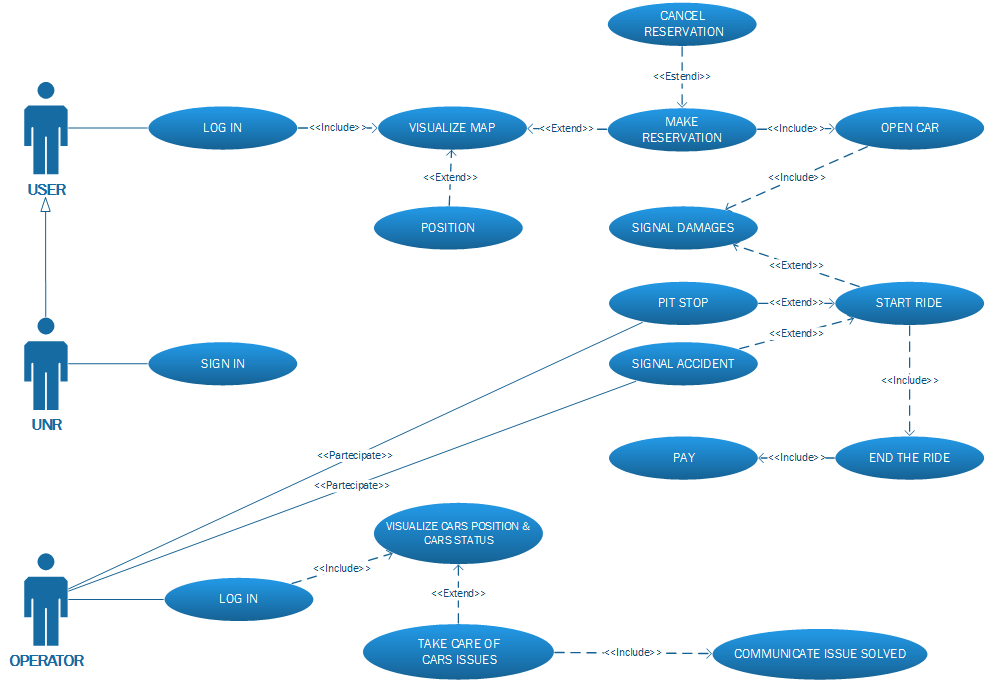
\includegraphics[width=10cm, height=10cm]{usecase}
\textbf{ Use case Description}\\
In this paragraph some use cases will be described. These use cases can be derived from the scenarios and the use case diagram. \\


\begin{center}
    \begin{tabular}{ | l | p{10cm}  |}
    \hline
    \textbf{Name} &  \textbf{Log in} \\ 
    \hline
    
    Description & A user logs into the system logs in
     \\ 
     \hline
    Actors & User
  \\ 
  \hline
    Entry Conditions & The user must be registered into the system \\ 
    \hline
    Flow of events & \begin{itemize}  \item A user opens the user?s log in page in the web or mobile app   \item The user inputs his credentials, consisting of a username and a password \item The user clicks on the ''LOG IN''  button \item The system checks that the credentials are valid (they are associated to an existing user) and redirects the user to the User?s Home page \end {itemize}  \\
    \hline
    Exit conditions & The user is redirected to the User?s home page.\\
    \hline
    Exceptions & If the username or password inserted by the user are not valid, the system does not redirect the user to the user?s home page. Instead, it notifies him that the credentials he inserted are not valid and tells him to try again\\
    \hline
    \end{tabular}
\end{center}


\begin{center}
    \begin{tabular}{ | l | p{10cm}  |}
    \hline
    \textbf{Name} &  \textbf{User visualizes a map of the cars} \\ 
    \hline
    
    Description & A user visualizes a geographical map where are enlighten the current positions of all available cars
     \\ 
     \hline
    Actors & User
  \\ 
  \hline
    Entry Conditions &  \\ 
    \hline
    Flow of events &
     \begin{itemize} 
      \item  The user can visualize from the user?s home page, directly accessible from the login page, a map of Milan?s urban area, where are enlighten the current geographical positions of all the available cars 
     
       \end {itemize}  \\
    \hline
    Exit conditions & The user is now aware of the positions of all the available cars (i.e. cars which can be reserved)\\
    \hline
    Exceptions & none\\
    \hline
    \end{tabular}
\end{center}


\begin{center}
    \begin{tabular}{ | l | p{10cm}  |}
    \hline
    \textbf{Name} &  \textbf{Location of cars whiten 1 km from a given position} \\ 
    \hline
    
    Description & A user inserts specific location and visualize all near available cars
     \\ 
     \hline
    Actors & User
  \\ 
  \hline
    Entry Conditions &  The user must be logged in \\ 
    \hline
    Flow of events &
     \begin{itemize} 
      \item  The user inputs a geographical location (consisting of a street/postal code/building etc.) into an input area at the bottom of the user?s home page
       \item  The user clicks on the ?SUBMIT? button
       \item The system dynamically changes the geographical area shown on the map,  in order to highlight the cars within 1 km from the location inserted by the user
       \item  
       \end {itemize}  \\
    \hline
    Exit conditions & The user can now see highlighted on the map the cars near the location he inserted\\
    \hline
    Exceptions & The user can now see highlighted on the map the cars near the location he inserted \\
    \hline
    \end{tabular}
\end{center}


\begin{center}
    \begin{tabular}{ | l | p{10cm}  |}
    \hline
    \textbf{Name} &  \textbf{Car reservation} \\ 
    \hline
    
    Description & The user can now see highlighted on the map the cars near the location he inserted
     \\ 
     \hline
    Actors & User
  \\ 
  \hline
    Entry Conditions &  The user can now see highlighted on the map the cars near the location he inserted\\ 
    \hline
    Flow of events &
     \begin{itemize} 
      \item  The user select a car on the map, among the available cars shown.
       \item  The system shows a ?RESERVE CAR" button near the selected car
       \item The user clicks on the ?RESERVE CAR? button
       \item  The system reserves a car for the user, making it unavailable to others, and redirects him to the reservation page, where he can visualize a message confirming that the reservation has been successful and a timer that shows the remaining minutes before the reservation expires, the position of the car etc 
       \end {itemize}  \\
    \hline
    Exit conditions & The user is redirected to the reservation page, where he can visualize the details of his reservation.\\
    \hline
    Exceptions & In case problems occur on the reservation process, an error message is shown, and the car remains available for other reservations\\
    \hline
    \end{tabular}
\end{center}


\begin{center}
    \begin{tabular}{ | l | p{10cm}  |}
    \hline
    \textbf{Name} &  \textbf{Reservation cancellation} \\ 
    \hline
    
    Description & In case problems occur on the reservation process, an error message is shown, and the car remains available for other reservations
     \\ 
     \hline
    Actors & User
  \\ 
  \hline
    Entry Conditions & The user must be logged into the system, and must have successfully reserved a car \\ 
    \hline
    Flow of events &
     \begin{itemize} 
      \item  From the reservation page, the user is able to visualize a ?CANCEL RESERVATION? button
       \item  The user clicks on the ?CANCEL RESERVATION ? button
       \item The system cancels the reservation, making the car available to other users
       \item  The system shows a message to inform that the reservation has been correctly cancelled
       \item The system redirects the user to the user?s home page
       \end {itemize}  \\
    \hline
    Exit conditions & The user is redirected to the User?s home page\\
    \hline
    Exceptions & None\\
    \hline
    \end{tabular}
\end{center}


\begin{center}
    \begin{tabular}{ | l | p{10cm}  |}
    \hline
    \textbf{Name} &  \textbf{Open car} \\ 
    \hline
    
    Description & A user opens the car he reserved
     \\ 
     \hline
    Actors & User
  \\ 
  \hline
    Entry Conditions & The user must have logged into the system and have successfully reserved a car. The user has reached the car he reserved and has the contactless card needed to unlock the car with him \\ 
    \hline
    Flow of events &
     \begin{itemize} 
      \item  The user places his contactless card near the car sensor before the timer expires
       \item  The system retrieves the information about the card and verifies that it corresponds to the user that reserved that car
       \item The system unlocks the car
       \item  
       \end {itemize}  \\
    \hline
    Exit conditions & The user has successfully unlocked the car \\
    \hline
    Exceptions & 
    \begin{itemize}
    \item If the timer has expired by the time the user places the contactless card near the car sensor, the system denies access to the car, notifying the user with a message on the mobile app and with a red light appearing on the car
    \item If the contactless the user uses to try unlock the car is not belonging to him, the system denies access to the car and notifies the user with a red light appearing on the car
    \item If the car the user tries to unlock is not the one he reserved, the system denies access to the car and notifies the user with a red light appearing on the car 
    \end{itemize}
    \\
    \hline
    \end{tabular}
\end{center}


\begin{center}
    \begin{tabular}{ | l | p{10cm}  |}
    \hline
    \textbf{Name} &  \textbf{Car issue signaling} \\ 
    \hline
    
    Description & A user communicate o the system weather there are issues on the car he reserved or not
     \\ 
     \hline
    Actors & User
  \\ 
  \hline
    Entry Conditions & The user has successfully reserved and unlocked a car \\ 
    \hline
    Flow of events &
     \begin{itemize} 
      \item  The system reminds the user to check for issues on the car with a message on the onboard computer before letting the user start the ride
       \item  The user checks if there are issues and do not find any
       \item The user taps on a button ?NO ISSUES FOUND? on the on-board computer
       \item  The system let the user know he can start the ride with a message on the on-board computer
       \end {itemize}  \\
    \hline
    Exit conditions & The user can now start the ride \\
    \hline
    Exceptions &  If the user find issues on the car, he communicate it to the system tapping a ?ISSUES FOUND? button on the on-board computer. The system cancels the reservation, making the car not available to the current user as well as all the others. The system tells the user to leave the car with a message on the on-board computer. The user is unable to start the ride and leaves the car. The system informs operators about the issue by marking the car as ?ASSISTANCE NEEDED?. \\
    \hline
    \end{tabular}
\end{center}


\begin{center}
    \begin{tabular}{ | l | p{10cm}  |}
    \hline
    \textbf{Name} &  \textbf{Start the ride} \\ 
    \hline
    
    Description & A user starts a ride with the car he reserved and unlocked
     \\ 
     \hline
    Actors & User
  \\ 
  \hline
    Entry Conditions & The user has successfully reserved and unlocked a car,  found no issues on that car and communicated it to the system.  \\ 
    \hline
    Flow of events &
     \begin{itemize} 
      \item  The user inserts and turns the car key and starts the engine
       \item  The user starts to be charged by the system
       \item The user starts to be able to visualize the updated amount of money spent for the ride on the on-board computer
       \item 
       \end {itemize}  \\
    \hline
    Exit conditions & The user successfully started the ride \\
    \hline
    Exceptions & None\\
    \hline
    \end{tabular}
\end{center}


\begin{center}
    \begin{tabular}{ | l | p{10cm}  |}
    \hline
    \textbf{Name} &  \textbf{Pit stop} \\ 
    \hline
    
    Description & The user makes a pit stop
     \\ 
     \hline
    Actors & User
  \\ 
  \hline
    Entry Conditions & The user has correctly started a ride on a car he reserved and unlocked \\ 
    \hline
    Flow of events &
     \begin{itemize} 
      \item  The user parks the car and stops the engine turning the key
       \item  The user taps on the ?START PIT STOP? button on the on-board computer
       \item The user starts to be charged by the system for half the price of a normal ride 
       \item  The user can now leave the car parked for maximum 60 minutes, keeping it reserved for future use
       \item The user gets back to the car, unlocks the car placing his contactless card near the car sensor
       \item The user taps on the ? END PIT STOP? button placed on the on-board computer
       \item The system restarts to charge the user for the full price as soon as the user taps on the ? END PIT STOP? button , and the user is able to restart the engine and continue to ride the car
       \end {itemize}  \\
    \hline
    Exit conditions & The user has successfully made a pit stop\\
    \hline
    Exceptions & In case the timer of 60 minutes expires by the time the user unlocks the car again in order to end the pit stop, the reservation for the car is cancelled, the system stops to charge the current user and makes the car available for other users. \\
    \hline
    \end{tabular}
\end{center}


\begin{center}
    \begin{tabular}{ | l | p{10cm}  |}
    \hline
    \textbf{Name} &  \textbf{End the ride} \\ 
    \hline
    
    Description & The user ends a ride
     \\ 
     \hline
    Actors & User
  \\ 
  \hline
    Entry Conditions & The user must have successfully started a ride  \\ 
    \hline
    Flow of events &
     \begin{itemize} 
      \item  The user parks the car and stops the engine turning the key
       \item  The user taps on the ?END THE RIDE? button on the on-board computer
       \item The system stops charging the user
       \item  The system reminds the user to close the windows and to leave the car in the same conditions in which he found it at the beginning of the ride with a message on the on-board computer
       \end {itemize}  \\
    \hline
    Exit conditions & The user has successfully ended a ride\\
    \hline
    Exceptions & None\\
    \hline
    \end{tabular}
\end{center}


\begin{center}
    \begin{tabular}{ | l | p{10cm}  |}
    \hline
    \textbf{Name} &  \textbf{Accident} \\ 
    \hline
    
    Description & A user reports an accident he is involved in while riding the car
     \\ 
     \hline
    Actors & User
  \\ 
  \hline
    Entry Conditions &  The user must have successfully started a ride\\ 
    \hline
    Flow of events &
     \begin{itemize} 
      \item  The user taps on the ?REPORT ACCIDENT? button on the on-board computer, which is available to press once the ride is started
       \item  The system marks the car as ?accident? and at the same time makes a call start from the on-board computer to allow the user to talk to an operator in order to provide the details of the accident and receive instructions.
       \item The operator that has been called taps on the ?OPERATE? button  on the row of the list associated to that car and provides assistance to the user.
       \item  Once the issue is resolved , the operator taps on the ?ISSUE SOLVED? on the same row of the list.
       \item The system marks back the car as ?NO ISSUE? 
       \end {itemize}  \\
    \hline
    Exit conditions & The user has successfully reported an accident to the operator, and the operator provided assistance.\\
    \hline
    Exceptions & None \\
    \hline
    \end{tabular}
\end{center}


\begin{center}
    \begin{tabular}{ | l | p{10cm}  |}
    \hline
    \textbf{Name} &  \textbf{Operator log in} \\ 
    \hline
    
    Description & An operator logs into the system
     \\ 
     \hline
    Actors & Operator
  \\ 
  \hline
    Entry Conditions & None \\ 
    \hline
    Flow of events &
     \begin{itemize} 
      \item  An operator opens the operator?s log in page on the web or mobile app
       \item  The operator inputs his credentials, consisting of a username and a password
       \item The operator clicks on the ?LOG IN? button
       \item  The system checks that the credentials are valid (they are associated to an existing operator) and redirects the operator to the Operator?s Home page
       \end {itemize}  \\
    \hline
    Exit conditions & The operator has successfully logged into the section of the system dedicated to operators \\
    \hline
    Exceptions & If the credentials inserted by the operator are not valid, the system shows an error message, inviting to try again and doesn?t redirect the operator anywhere \\
    \hline
    \end{tabular}
\end{center}


\begin{center}
    \begin{tabular}{ | l | p{10cm}  |}
    \hline
    \textbf{Name} &  \textbf{Operator views cars information and takes care of a car} \\ 
    \hline
    
    Description & An operator visualizes the status and position of all the cars on a list
     \\ 
     \hline
    Actors & Operator
  \\ 
  \hline
    Entry Conditions & The operator must be logged into the system \\ 
    \hline
    Flow of events &
     \begin{itemize} 
      \item  The operator  visualizes from the Operator?s home page, directly accessible from the login page, a  table: each row of the table is associated to a car, and it features the position (expressed in terms of latitude and longitude, the status (consisting of  a writing among ?NO ISSUES?, ?ASSISTANCE NEEDED?, ?LOW CHARGE? and ?ACCIDENT?), the name of the user who is using the car and the ID of the car. The list also shows if other operators  already decided to take care of a car by showing a writing ?in progress? or a button ?OPERATE ?  on the rows associated to issued cars.
       \item  An operator taps on the ?OPERATE ? button related to a car which status is ?ASSISTANCE NEEDED?, ?LOW CHARGE? or ?ACCIDENT"
       \item After he took care of the issue,  the operator taps on the button ?ISSUE SOLVED? on the same row of the list, to communicate that the car is now back to its regular functions.
       \item  The system marks back the car as ?NO ISSUE?  
       \end {itemize}  \\
    \hline
    Exit conditions & The operator has successfully solved an issue of a car.\\
    \hline
    Exceptions & None \\
    \hline
    \end{tabular}
\end{center}



\subsection{Activity Diagrams} %ACTIVITY
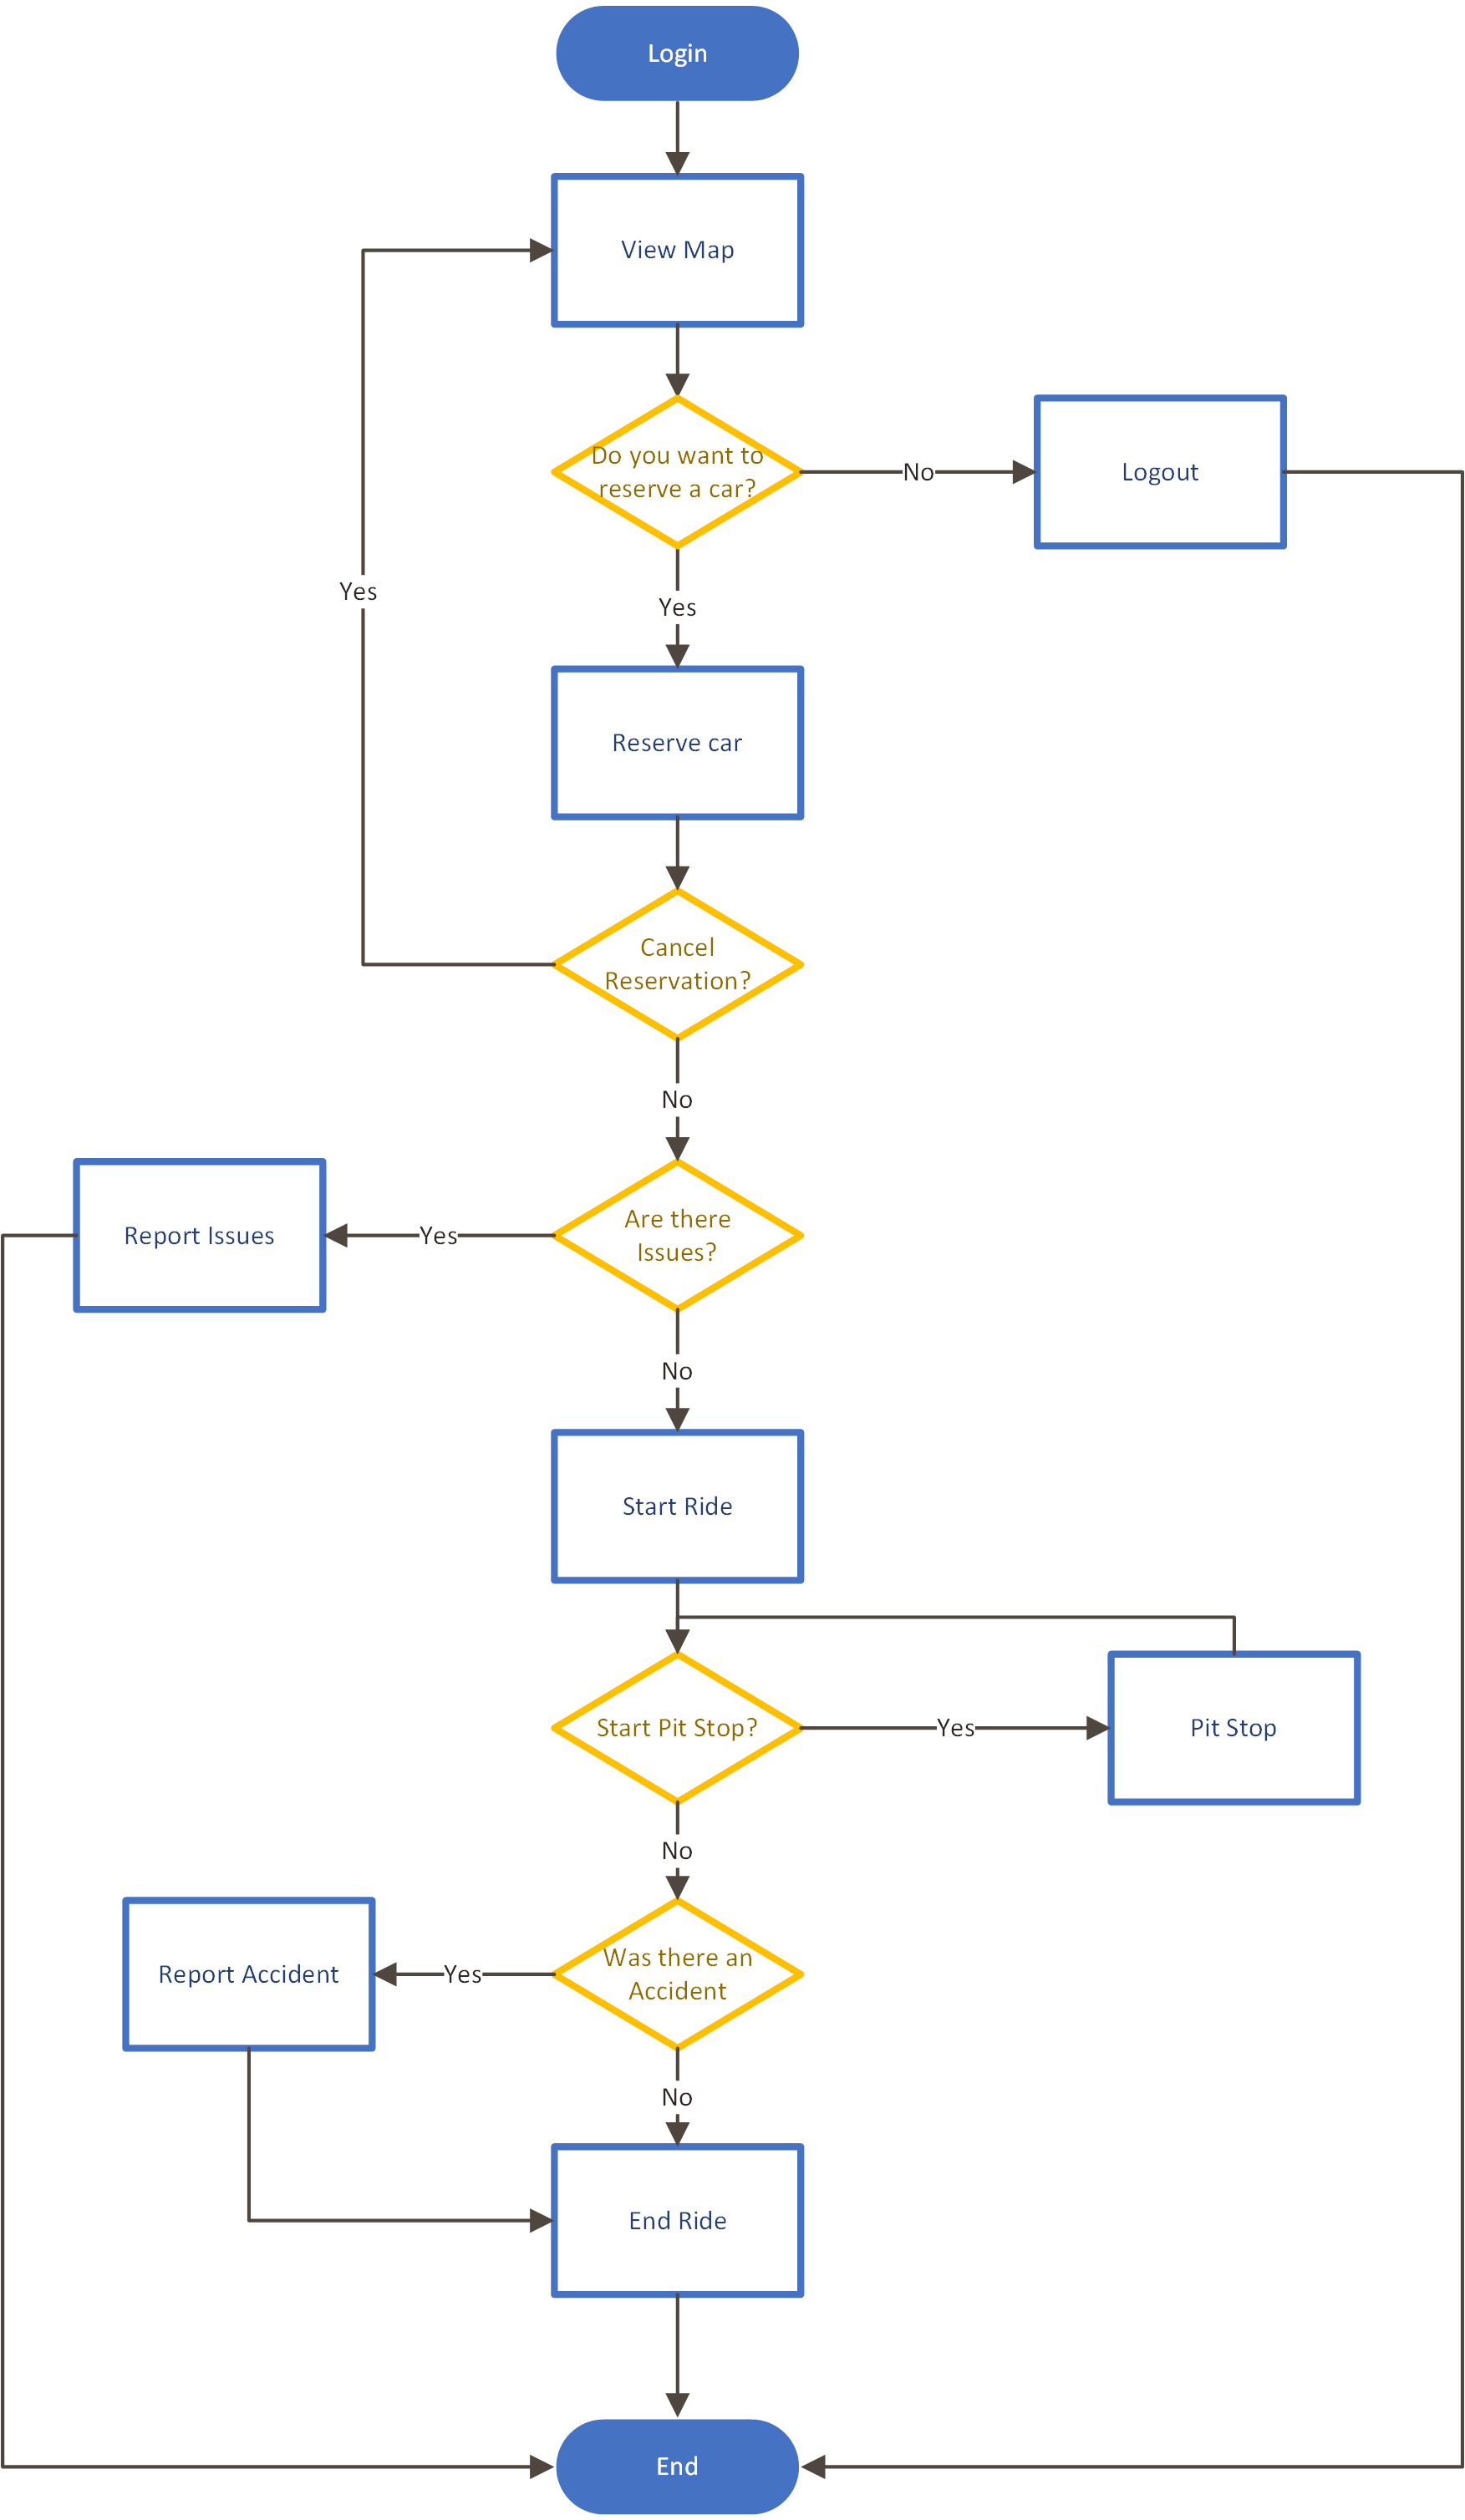
\includegraphics[width=13cm, height=20cm]{activity}
\subsection{Class Diagrams} %CLASS 
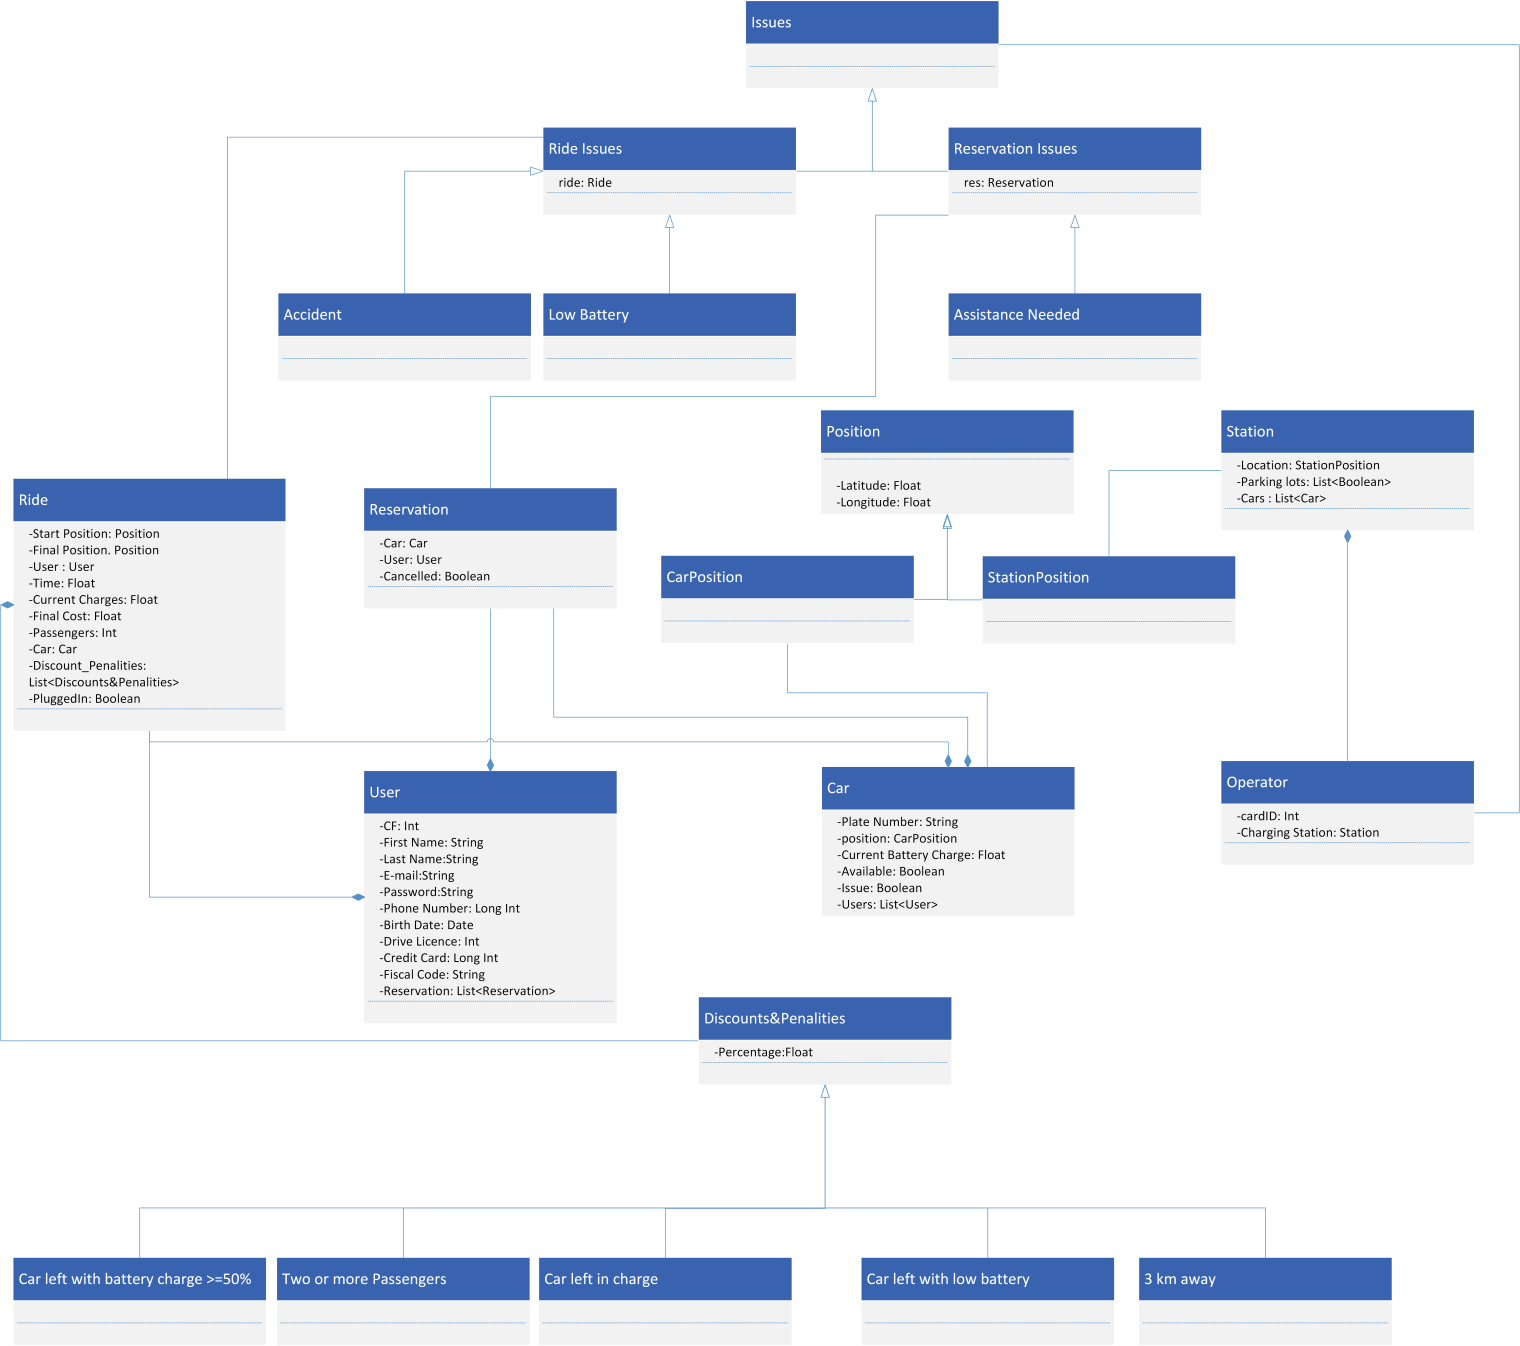
\includegraphics[width=13cm, height=20cm]{class}
\subsection{State Diagrams} %STATE
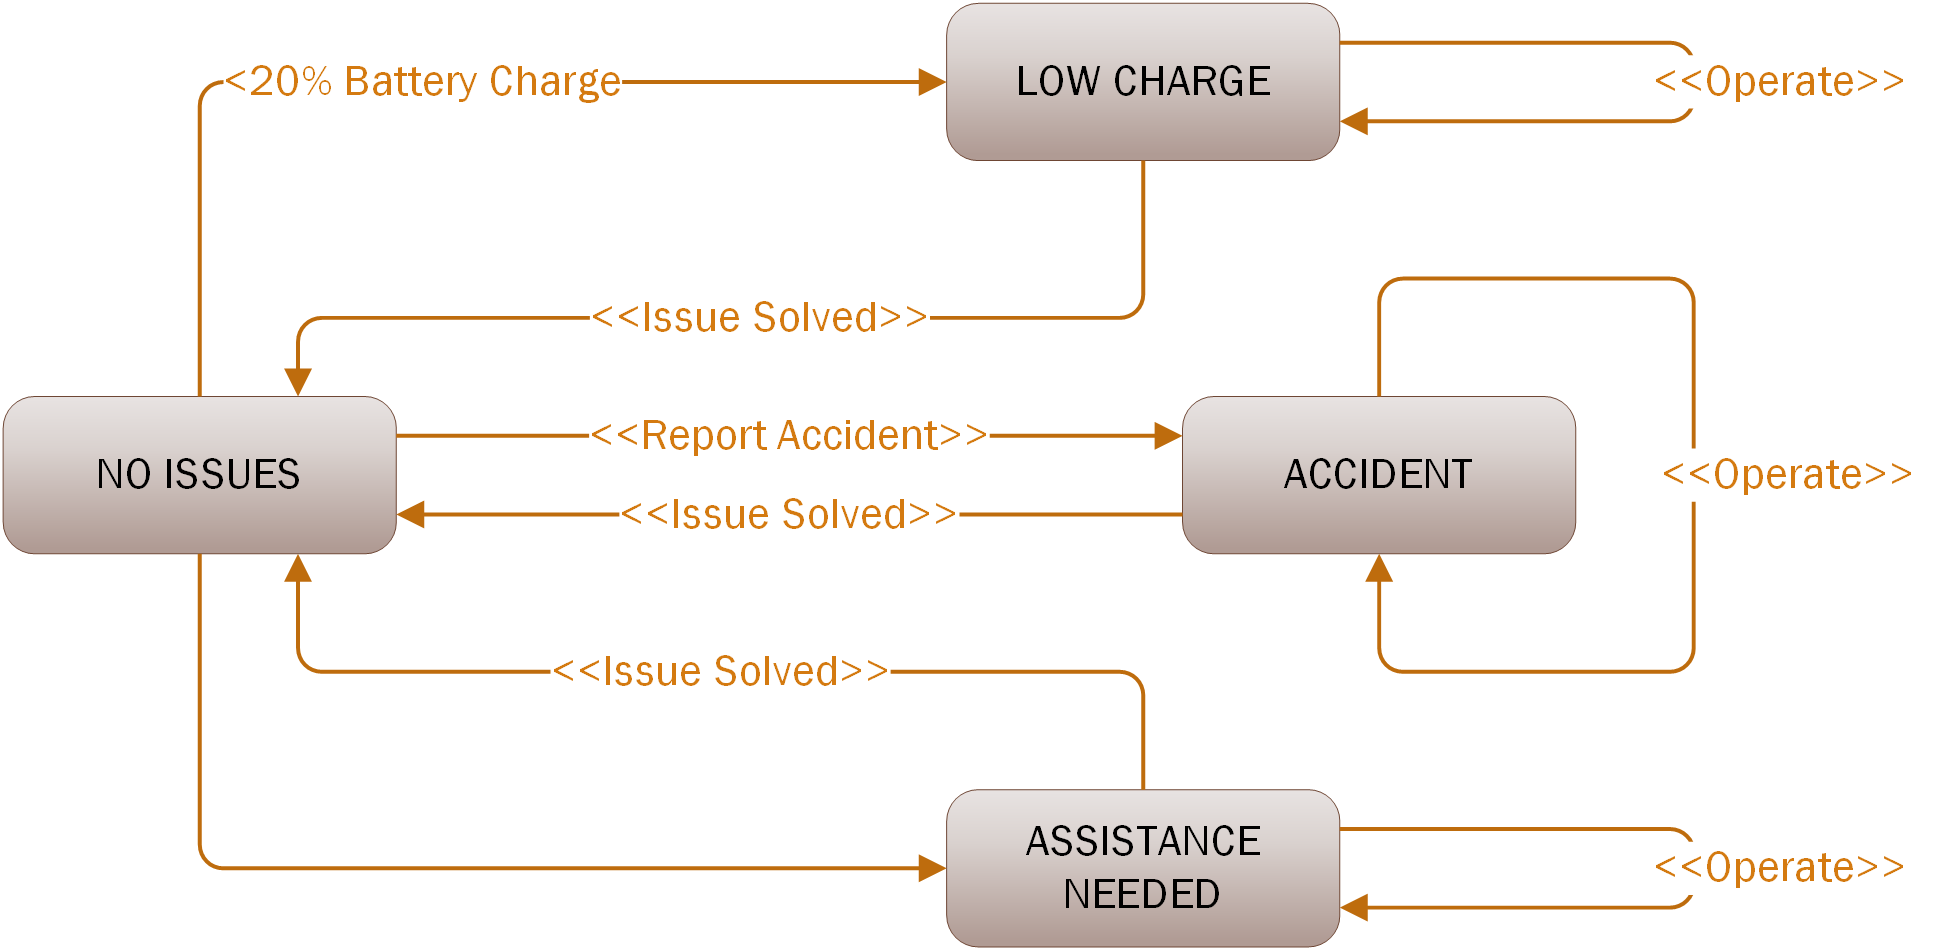
\includegraphics[width=13cm, height=10cm]{state}

\newpage
\subsection{Sequence Diagrams} %SEQUENCE
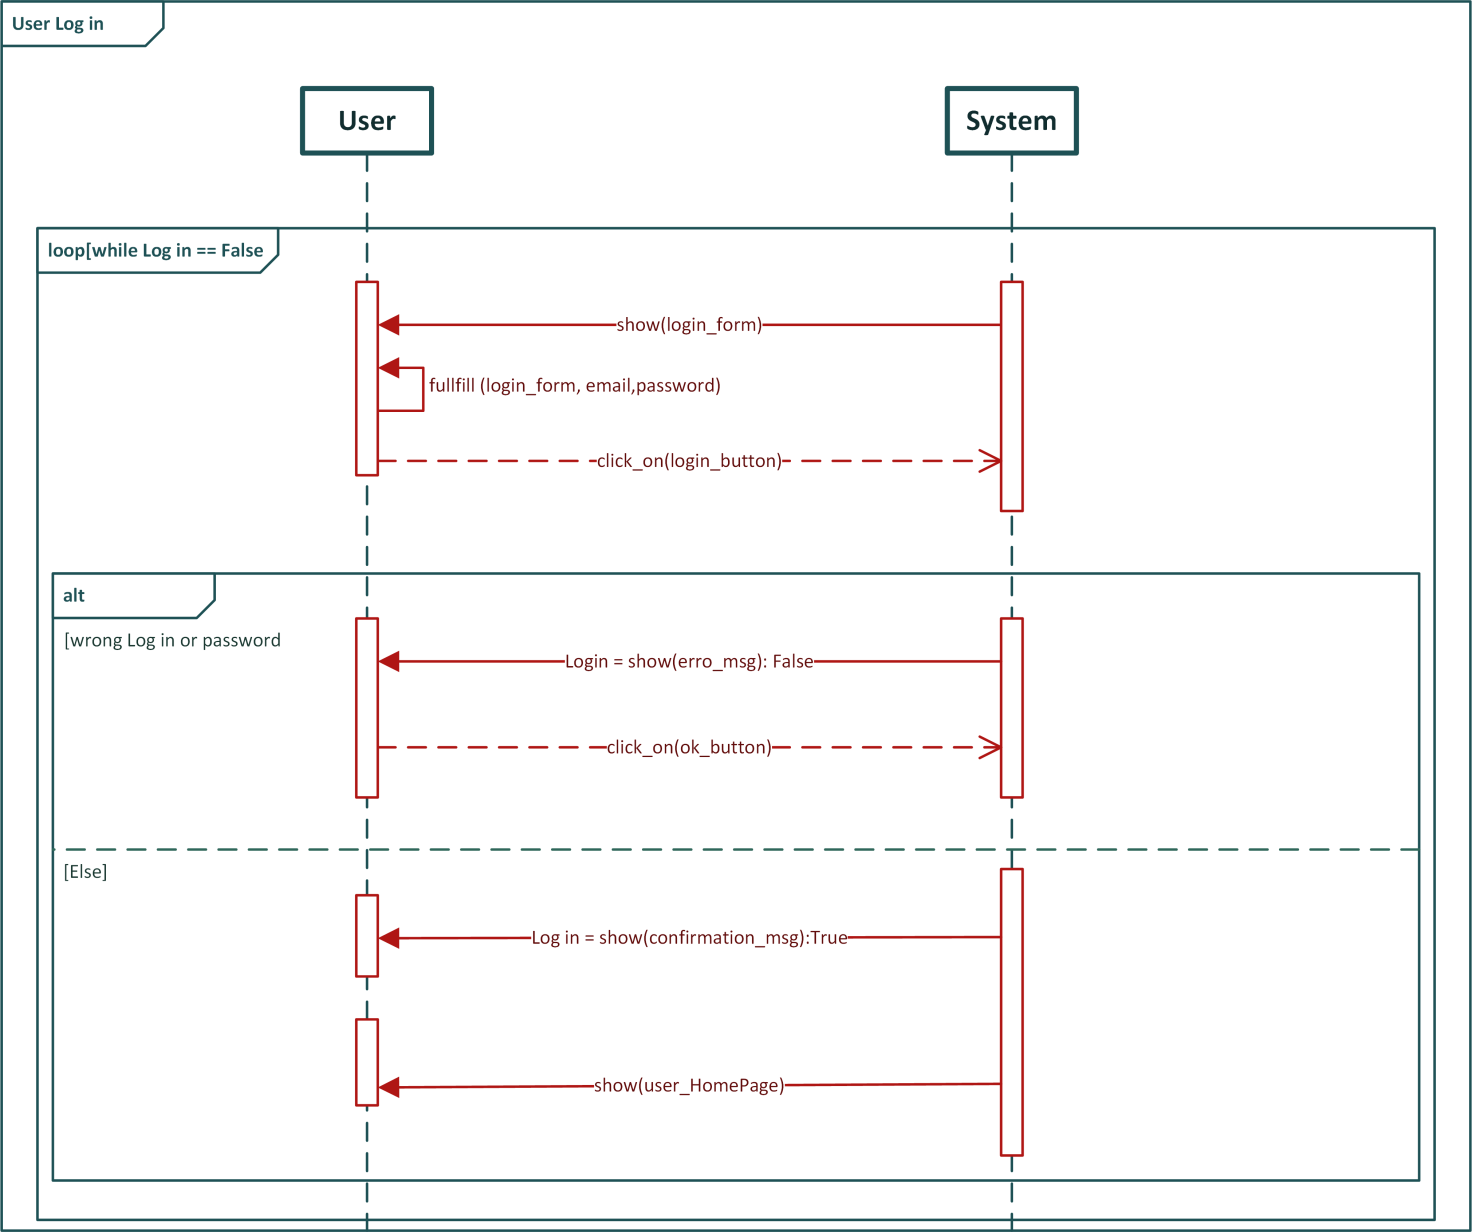
\includegraphics[scale=0.9]{seq1}
\newpage
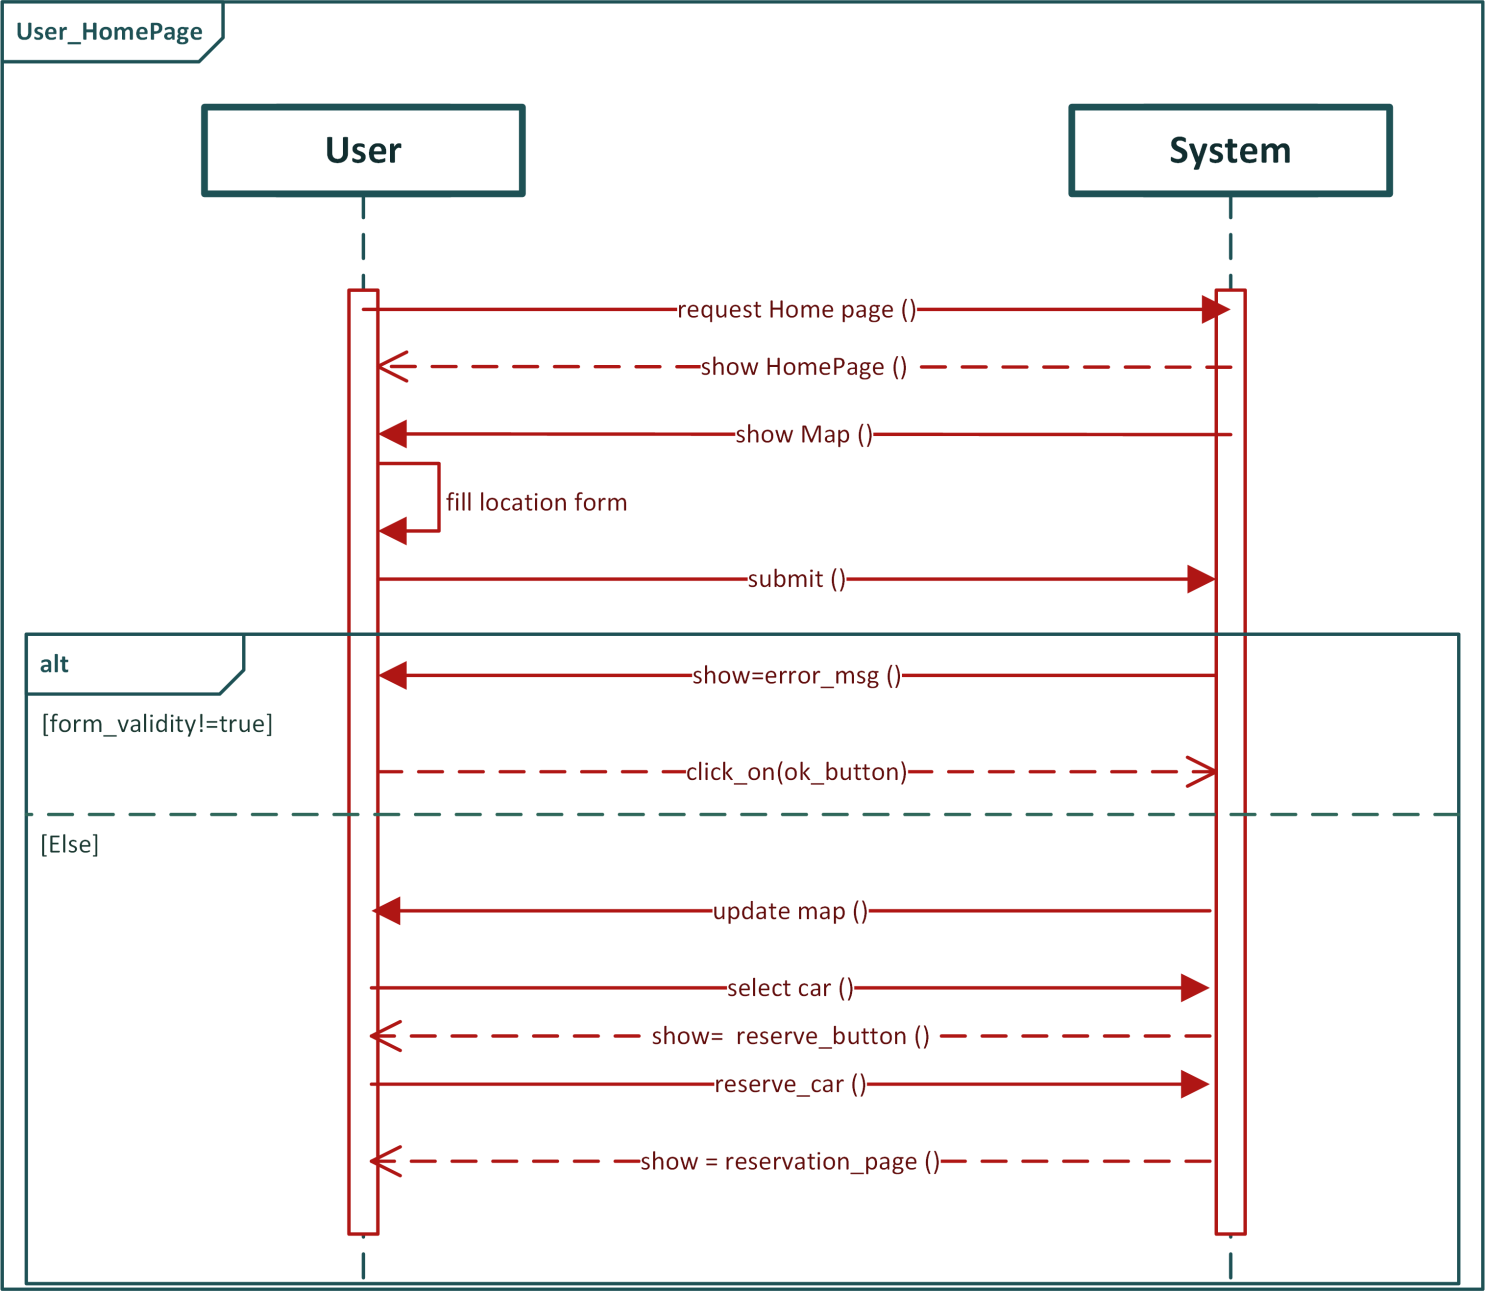
\includegraphics[scale=0.9]{seq2}
\newpage
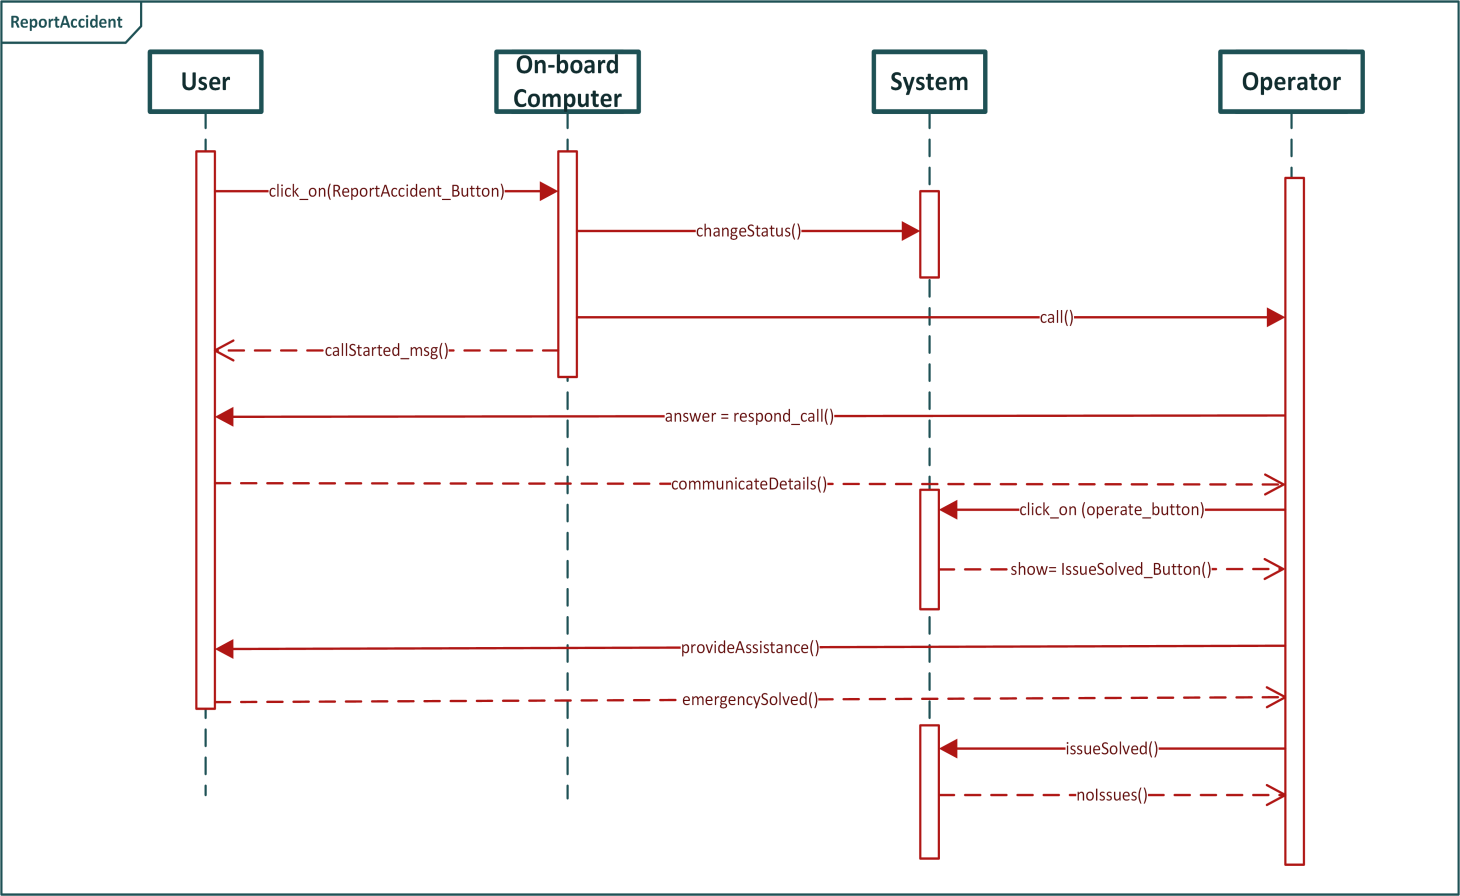
\includegraphics[scale=0.9]{seq3}
\newpage


\section{Alloy} %ALLOY
\subsection{Model} %MODEL
\begin{lstlisting}
open util/boolean

sig Email{}

sig User {
identifyby:Email,
}

fact UniqueEmail{
User.identifyby=Email
}

fact OneEmailperUser {
all u1,u2 : User | u1!=u2 => u1.identifyby != u2.identifyby
}

sig Car {
plate: Int,
position : CarPosition
}{plate>0}

fact OnlyOnePlatePerCar{
all c1,c2 :Car | c1!=c2 => c1.plate != c2.plate
}

fact UniqueCarPosition {
Car.position = CarPosition
}
fact OnlyOnePositionPerCar{
all c1,c2 :Car | c1!=c2 => c1.position != c2.position
}


sig Reservation {
reservedby: one User,
car: Car,
issue : lone ReservationIssue
}

fact UniqueRes {all r1,r2 :Reservation | 
r1!=r2 => r1.reservedby!=r2.reservedby}
fact UniqueCar{all r1,r2 :Reservation | r1!=r2 => r1.car!=r2.car }

fact AllReservationIssuesAreAssociatedToAReservation 
{ Reservation.issue = ReservationIssue}
fact NoReservationsAssociatedToTheSameIssue{ all r1, r2 : Reservation 
| r1!=r2 => r1.issue!=r2.issue}

sig Ride {
driveby:  one User,
car:Car,
passengers :Int ,
issue : set RideIssue ,
discountsPenalities : set DiscountPenalities
}{
passengers<5
passengers>1
#issue=1 or #issue =0
}

fact LowChargeIssueImpliesLowChargePenality  {
no r: Ride |  all i : LowCharge | all dp: CarWithLowCharge | 
 (dp in r.discountsPenalities && !(i in r.issue)) || 
(i in r.issue && !(dp in r.discountsPenalities))
 }
fact  LowChargeIssueImpliesNoPluggedInCar {
no r:Ride | some dp: CarWithLowCharge | some dp2: CarPluggedIn | 
 (dp in r.discountsPenalities) && (dp2 in r.discountsPenalities)
 }
fact LowChargeIssueImpliesNoChargedCar {
 no r: Ride | some dp: CarWithLowCharge | some dp2 : ChargedCar | 
 (dp in r.discountsPenalities) && (dp2 in r.discountsPenalities)
 }
fact morePassengerDiscountImpliesAtLeastThreePassengers {
all r:Ride | all dp: MorePassengers  | 
(dp in r.discountsPenalities) && r.passengers>2
}
fact d1 {
all r: Ride | all dp1: CarPluggedIn | all dp2:  CarWithLowCharge | 
dp1 in r.discountsPenalities <=>!(dp2 in r.discountsPenalities)
 }

fact AllDiscountsHaveARide {
Ride.discountsPenalities=DiscountPenalities 
}

fact d2 {
all r:Ride ,dp1 , dp2 : ThreeKmAway |  
dp1!=dp2 && dp1 in r.discountsPenalities <=>!(dp2 in r.discountsPenalities)
}
fact d2 {
all r:Ride, dp1, dp2 : CarWithLowCharge | 
dp1!=dp2 &&  dp1 in r.discountsPenalities <=>!(dp2 in r.discountsPenalities)
}
fact d2 {
all r:Ride, dp1, dp2 : CarPluggedIn |
 dp1!=dp2 && dp1 in r.discountsPenalities <=>!(dp2 in r.discountsPenalities)
}
fact d2 {
all r:Ride,  dp1, dp2 : ChargedCar | 
dp1!=dp2 && dp1 in r.discountsPenalities <=>!(dp2 in r.discountsPenalities)
}
fact d2 {
all r:Ride,  dp1, dp2 : MorePassengers | 
(dp1!=dp2 && dp1 in r.discountsPenalities) <=>!(dp2 in r.discountsPenalities)
}
fact AllRideIssuesAreAssociatedToARide { 
Ride.issue = RideIssue
} 
fact NoRidesAssociatedToTheSameIssue{
 all r1, r2 : Ride | r1!=r2 => r1.issue!=r2.issue
}
fact UniqueRide {
all r1,r2 :Ride | r1!=r2 => r1.driveby!=r2.driveby
}
fact UniqueRideCar {
all r1,r2 :Ride | r1!=r2 => r1.car!=r2.car
}
fact CarRideOrRes1 {
Ride.car = Ride.car - Reservation.car
}
fact CarRideOrRes2 {
Reservation.car= Reservation.car- Ride.car
}
fact ResOrRide {
Ride.driveby = Ride.driveby - Reservation.reservedby
}


fact ResOrRide1 {
Reservation.reservedby= Reservation.reservedby- Ride.driveby
 }

sig CardID{}

sig Operator{
id: CardID,
station :  one ChargingStation,
issueToTakeCareOf : lone Issues
}

fact everyIssueHasAnOperator { 
Operator.issueToTakeCareOf = Issues
}
fact DifferentOperatorsAssociatedToDifferentIssues {
 all o1, o2: Operator | o1!=o2 => o1.issueToTakeCareOf !=o2.issueToTakeCareOf
}
fact OneIDperOperator {
all o1,o2 : Operator | o1!=o2 => o1.id != o2.id
}
fact UniqueCardID{
Operator.id=CardID
}

sig ChargingStation {
position: StationPosition,   
}

fact UniqueWorker { 
Operator.station=ChargingStation
}
fact OnePositionPerStation {
all cg1, cg2 : ChargingStation | cg1!= cg2 => cg1.position != cg2. position
}
fact UniquePosition{
ChargingStation.position = StationPosition
}





abstract sig DiscountPenalities{}

abstract sig Discounts extends DiscountPenalities{}
abstract sig Penalities extends DiscountPenalities{}

sig MorePassengers extends Discounts{}
sig CarPluggedIn extends Discounts{}
sig  ChargedCar extends Discounts{}
sig  ThreeKmAway extends Penalities{}
sig  CarWithLowCharge extends Penalities{}

abstract sig Issues {}

abstract sig RideIssue extends Issues {}
abstract sig ReservationIssue extends Issues{}

fact ItsAlwaysIssuesWeAreTalkingAbout {
 RideIssue + ReservationIssue = Issues
} 


sig Accident extends RideIssue {}
sig AssistanceNeeded extends ReservationIssue {}
sig LowCharge extends RideIssue {}

fact AllRideIssues{ 
Accident + LowCharge = RideIssue
}

abstract sig Position{}
sig StationPosition extends Position {}
sig CarPosition extends Position {}

pred show {
#Ride = 1
#Reservation = 1
#User = 3
#ChargingStation = 1
#Operator = 2
}


assert everyOperatorDoesHisJob {
all r:Ride |all  i : RideIssue | some op: Operator | 
( i in r.issue) =>i in op.issueToTakeCareOf 
 } 
assert everyOperatorDoesHisJob2 {
all res: Reservation | all i: ReservationIssue | 
some op: Operator| (i in res.issue ) =>i in op.issueToTakeCareOf
}
assert everyRideLowChargeIssueHasALowChargePenality {
all r:Ride | some i: LowCharge | some dp: CarWithLowCharge | 
i in r.issue <=> dp in r.discountsPenalities
}
assert noLowChargeIssueOnPluggedInCars {
no r:Ride |some dp:CarWithLowCharge  | some i: LowCharge  | 
some dp2 : CarPluggedIn | 
(i in r.issue || dp in r.discountsPenalities) && (dp2 in r.discountsPenalities)
}
assert noLowChargeIssueChargedInCars {
no r:Ride |some dp:CarWithLowCharge  | some i: LowCharge  | 
some dp2 : ChargedCar | 
(i in r.issue || dp in r.discountsPenalities) && (dp2 in r.discountsPenalities)
}

check noLowChargeIssueChargedInCars
check noLowChargeIssueOnPluggedInCars
check everyOperatorDoesHisJob 
check everyOperatorDoesHisJob2 
check everyRideLowChargeIssueHasALowChargePenality
run show for 5 
\end{lstlisting}

\textbf{Alloy Result}
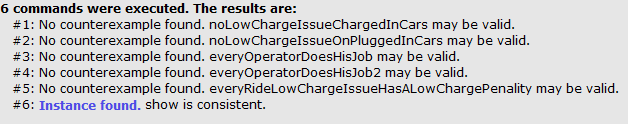
\includegraphics{result}


\subsection{World Generated} %WORLD
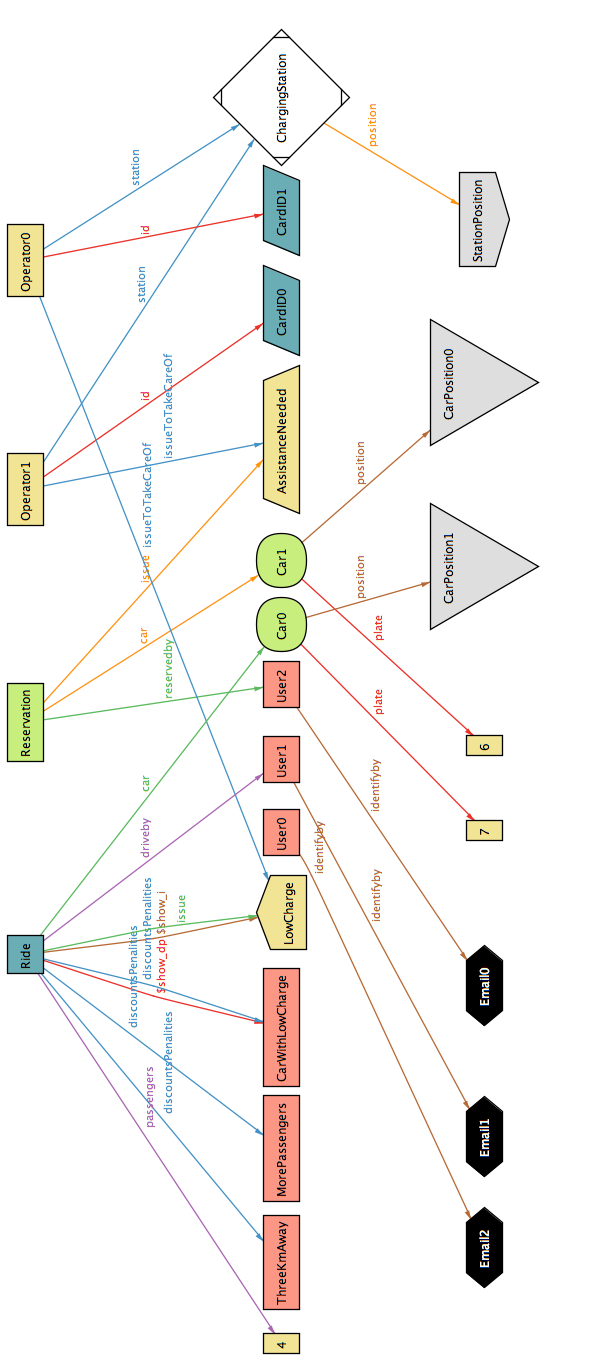
\includegraphics[width=13cm, height=20cm]{world}
\section{Other Features} %OTHGER FEATURES
\subsection{Future Development} %FUTURE DEVELOPMENT
We are thinking about extending  the perimeter of the safe area to the whole region, and possibly applying it to other regions.  We also plan to implement a more innovative and computationally efficient method to let the system check whether a car is parked within 3 km of distance from the nearest safe area , using a special signal created by emitters  placed into charging stations instead of  using the GPS sensor.
\subsection{Hours of work} %HOW
\textbf{Joshua Nicolay Ortiz Osorio }
\begin{itemize}
\item 26/10/2016 : 1h30m
\item 28/10/2016 : 2h30m
\item 29/10/2016 : 1h
\item 1/11/2016 : 2h 
\item 4/11/2016 : 2h
\item 5/11/2016 : 1h 
\item 8/11/2016 : 3h 
\item 9/11/2016 : 3h
\item 10/112016 : 3h
\item 11/11/2016 :2h30m 
\item 12/11/2016 : 4h 
\item 13/11/2016 : 4h 
\end{itemize}


\textbf{Michelangelo Medori }
\begin{itemize}
\item 26/10/2016 : 1h30m
\item 27/10/2016 : 2h
\item 29/10/2016 : 2h30m
\item 1/11/2016 : 2h 
\item 4/11/2016 : 2h 
\item 5/11/2016 : 1h
\item 8/11/2016 : 3h
\item 10/112016 : 3h
\item 11/11/2016 :2h30m
\item 12/11/2016 : 4h
\item 13/11/2016 : 4h

\end{itemize}

\subsection{Used Tools} %USED TOOLS
\begin{itemize}
\item Visio: for Use Case Diagram, Sequence Diagrams, State Diagram and Activity Diagram 
\item Balsamiq : to make mock-ups
\item Latex : to write the document and create .pdf
\item Github: for version controller
\item Alloy Analizer 4.2 . to prove the consistency of our model
\item Dropbox : to share documents online

\end{itemize}
\end{flushleft} %%%%%%%%%%%%%%%%%%%%%%%%%%%%%%%%%%%%%%%%%%%%%%
\end{document}